\documentclass{../../ece-report}

\usepackage{subcaption}
\usepackage{multirow}


\memostudent{Ty Davis}
\memotitle{Lab 7 - NMOS Based Source Follower}
\memocourse{ECE 3110}
\memodate{\today}


\newcommand{\Vsub}[1]{\ensuremath{\textnormal{V}_{#1}}}
\newcommand{\sub}[2]{\ensuremath{\textnormal{#1}_{#2}}}

\renewcommand{\half}{\frac{1}{2}}



\begin{document}

\maketitle

\section{Introduction and Theory}

Similar to the last lab, we are going to select resistors
to design an amplifier. This time, however, we are designing
a \emph{Source Follower} configuration of a MOSFET amplifier. 
It is also known as the common drain, because the drain 
lead of the transistor is the common reference for the other
leads.

Fig.~\ref{fig:circuit_full} shows the entire circuit.
We are going to design the circuit such that $I_D =
1~\si{\mA}$ and $A_v = 0.8~\si{\V/\V}$. Also, we are
given that $R_\textnormal{sig} = 50~\si{\ohm}$ and $R_G = 10~\si{\kohm}$.



\begin{figure}[h!]
  \centering
    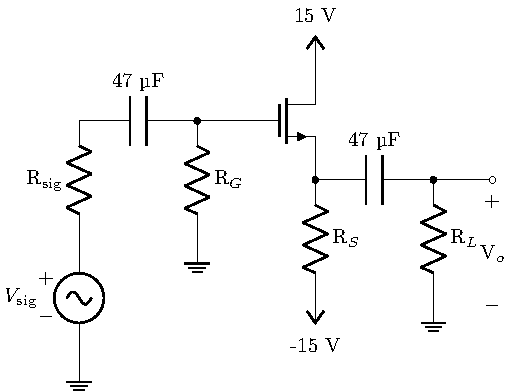
\includegraphics{../circuits/circuit_full.pdf}
  \caption{The circuit that we are analyzing in this lab.}\label{fig:circuit_full}
\end{figure}

\section{DC Analysis}

To start off, we need to find the correct value of $R_S$
to bias the transistor properly. For DC analysis, we
can assume that the capacitors act as open circuits,
and the remaining circuit is shown in Fig.~\ref{fig:circuit_dc}.

\begin{figure}[h!]
  \centering
    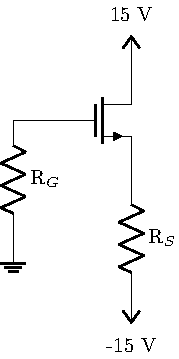
\includegraphics{../circuits/circuit_dc.pdf}
  \caption{The circuit after removing the capacitors.}\label{fig:circuit_dc}
\end{figure}

Knowing that $I_D = 1~\si{\mA}$, and using this equation:

\[
  V_{GS} = \sqrt{\frac{2 I_D}{k_n}} + V_{th}
\]

we can obtain a value for $V_{GS}$. Remember from the
previous labs that $k_n = 70.3~\si{\mA / \V ^2}$, and
$V_{th} = 2.1~\si{\V}$. This yields $V_{GS} = 2.269~\si{\V}$.

Without out any current flowing through the gate of
the transistor, the voltage $V_G=0~\si{\V}$, and thus
$R_S = 12.731~\si{\kohm}$. It's good to note right now
as well that $V_{ov} = 0.169~\si{\V}$.

\section{AC Analysis}

Fig.~\ref{fig:circuit_t_model} shows the circuit as
it can be used for the AC analysis. The transistor
has been replaced by the \emph{T Model}, and the capacitors
have all been swapped for short circuits.

Seeing the circuit this way can help for small signal analysis.
We are designing the circuit such that $A_v = 0.8~\si{\V/\V}$, and
we know that $A_v = \frac{v_o}{v_i}$. Looking at the circuit
with the T Model we can see derive the following voltage divider:

\[
  v_o = v_i \frac{R_L \| R_S}{1/g_m + R_L \| R_S}
\]


Using $g_m = k_n V_{ov}$, we find $g_m = 11.8~\si{\m\siemens}$, which
allows us to find $R_L \| R_S = 336.68~\si{\ohm}$.

With the calculated $R_S$ from the DC analysis, $R_L$
is then equal to $R_L = 345.8~\si{\ohm}$.

The output $R_o$ looking into the amplifier is clearly
shown with the T Model, and is simply just $R_o = 1/g_m$.

It's good to note as well, that the ratio of $R_G$ to $R_\textnormal{sig}$ is
so large that you can essentially approximate $v_i = v_\textnormal{sig}$.

\begin{figure}[h!]
  \centering
    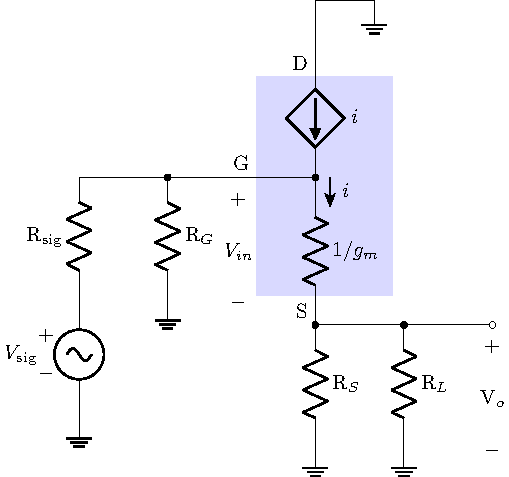
\includegraphics{../circuits/circuit_t_model.pdf}
  \caption{The T Model equivalent circuit with capacitors replaced by shorts.}\label{fig:circuit_t_model}
\end{figure}


\section{Simulation}

Simulating the circuit with Multisim was straightforward, and the results are
shown in Fig.~\ref{fig:sim}. The gain was simulated at $A_v = 0.82~\si{\V/\V}$.

The DC operating points were: $V_G = 450~\si{\nV}$,
$V_{GS} = 2.13~\si{\V}$, $V_{DS} = 17.14~\si{\V}$, and 
$I_D = 0.997~\si{\mA}$.

\begin{figure}[h!]
  \centering
  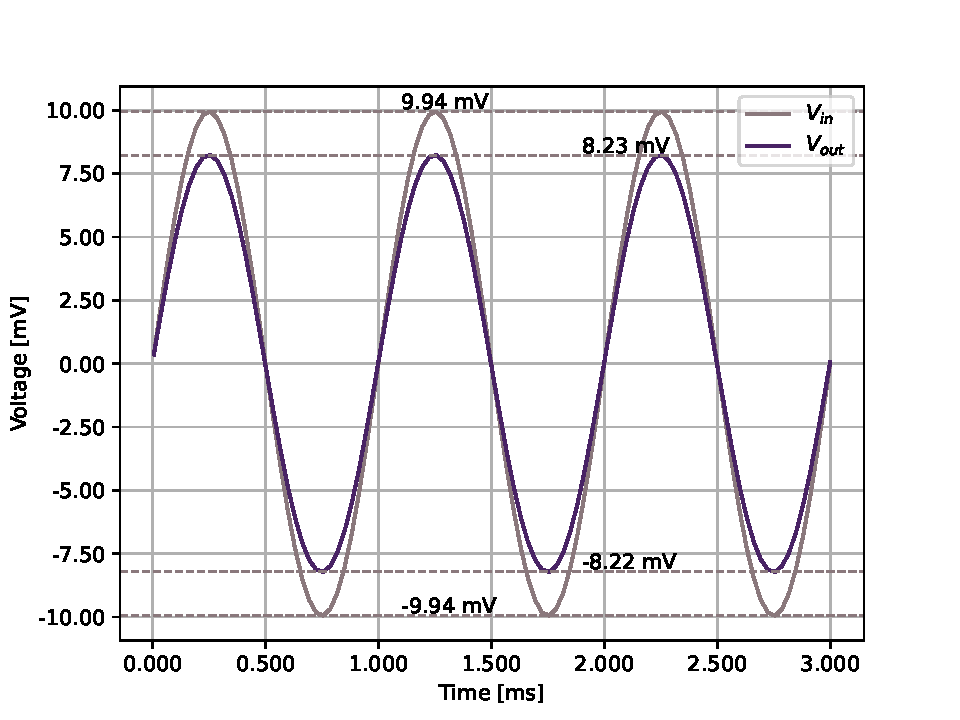
\includegraphics[width=0.6\textwidth]{../plots/pdf/sim.pdf}
  \caption{Simulation Results.}\label{fig:sim}
\end{figure}

\section{Results}

Building and Measuring the circuit showed that our calculations
and simulation were accurate. 

The DC operating points were found at $V_G = 0~\si{\V}$,
$V_{GS} = -1.89~\si{\V}$, $V_{DS} = 16.89~\si{\V}$,
and $I_D = 1.04~\si{\mA}$ was calculated from the corresponding
values and the measured resistance. All the measured resistors are 
shown in Table~\ref{tab:resistors}.

Fig.~\ref{fig:meas} shows the input vs output waveform, and
the measured gain was $A_v = 0.748~\si{\V/\V}$.


\begin{figure}[h!]
  \centering
  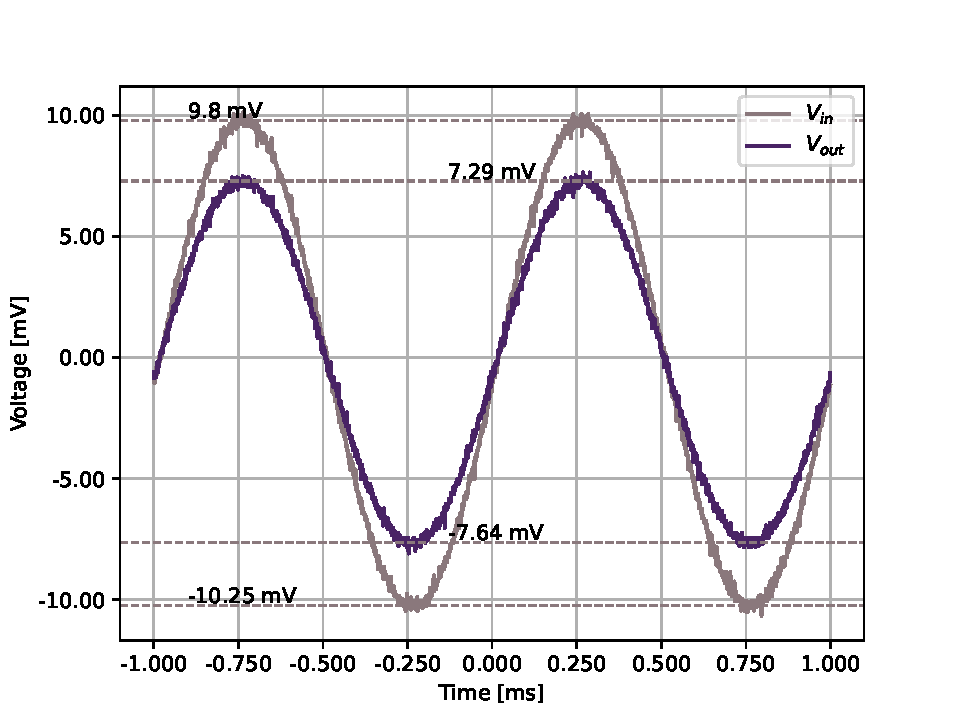
\includegraphics[width=0.6\textwidth]{../plots/pdf/meas.pdf}
  \caption{Measurement Results.}\label{fig:meas}
\end{figure}

\begin{table}[h!]
  \centering
  \begin{tabular}{l l l c}\toprule
    \textbf{Calculated Resistor} & \textbf{Equivalent Resistor} & \textbf{Measured Resistor} & \\
    \midrule

12.731 \si{\kohm} & 12.691 \si{\kohm} & 12.517 \si{\kohm} & $R_S$ \\
          & 100 \si{\kohm}    & 98.8 \si{\kohm}   &       \\
          & 15 \si{\kohm}     & 14.79 \si{\kohm}  &       \\
          & 470 \si{\kohm}    & 464.1 \si{\kohm}  &       \\
          \midrule
345 \si{\ohm}    & 340 \si{\ohm}    & 334 \si{\ohm}    & $R_D$ \\
          & 10 \si{\ohm}     & 9.84 \si{\ohm}   &       \\
          & 330 \si{\ohm}    & 324   \si{\ohm}  &       \\
          \midrule
10 \si{\kohm}     & 10 \si{\kohm}     & 9.86 \si{\kohm}  & $R_G$ \\
\bottomrule
\end{tabular}
\caption{Measured resistors.}
\label{tab:resistors}
\end{table}

\section{Post-Measurement Exercise}

Some of the answers were included in the \textbf{Results} section, but
the remaining questions are answered here.

Q. What would happen if you used the function generator
with 50\si{\ohm} output resistance to directly drive
your load resistor?

A. Without the buffer amplifier, the output signal would
be attenuated to according to the voltage divider with
the signal resistance and the 340~\si{\ohm} load resistance.
The corresponding gain would be about $A_v = 0.87$.
That's comparable to our circuit.

Q. What would happen if the output resistance of the
function generation was changed from 50~\si{\ohm} to
5~\si\kohm?

A. With a much larger input resistance, the signal is
significantly attenuated according to a much more extreme
voltage divider. The resulting gain would be $A_v =
0.064$, which is very poor. Using the buffer circuit prevents this.

\end{document}
